\section{Gaussian Channel}
一个信号 $x(t)$ 的能量和功率为
\begin{align*}
E &= \int_{-\infty}^{\infty} x^2(t) \dt \\
P &= \lim_{T\to\infty} \dfrac{1}{T}\int_{-\frac{T}{2}}^{\frac{T}{2}} x^2(t) \dt
\end{align*}
当传输为离散时, 采样点为 $X_1,\ldots, X_n\stackrel{i.i.d.}{\sim} X$, 由大数定理可得:
$$P = \lim_{T\to\infty} \dfrac{1}{T}\sum_{n=-\frac{T}{2}}^{\frac{T}{2}} X_i^2\to \mathbb{E}(X^2)$$
信道在传输信号时有传输功率 $P$ 的限制. 所以我们可以用 $\mathbb{E}(X^2)\leq P$ 作为信号的传输功率限制. 因为平移不会改变信息熵, 所以不妨设$X$的均值为$0$以减少能量的浪费, 此时约束变为 $\Var(X)\leq P$.
\begin{figure}[htbp]
    \centering
    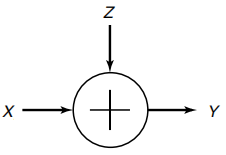
\includegraphics[width=0.4\textwidth]{./figures/chapter7/Gaussian_channel.png}
\end{figure}

高斯信道如下图所示. 其中$X$为信道的输入, 传输过程中有噪声$Z \sim \mathcal{N}(0, N)$, 且$X\perp Z$. 信道的输出为$Y = X + Z$. 高斯信道又叫 Additive White Gaussian Noise (AWGN) 信道.

由于信道容量$C$为每次可靠传输的bit数, 所以$N=0$时$C=+\infty$. 若$X$传输时没有功率限制, 则$C=+\infty$. 但是在考虑真实的高斯信道时加上$\Var(X)\leq P$的限制.

由上一章可知, Gaussian的方差为$\sigma^2$时的熵为$h(X) = \dfrac{1}{2}\ln(2\pi e \sigma^2)$ nats. 所以当 $X\sim \mathcal{N}(0, P)$ 时, $Y\sim \mathcal{N}(0, P+N)$, $Y|X\sim \mathcal{N}(X, N)$, 此时有
$$I(X;Y) = h(Y) - h(Y|X) = \dfrac{1}{2}\ln\left(1+\dfrac{P}{N}\right) \text{ nats}$$
后面我们证明这其实就是高斯信道的信道容量.

\begin{example}
A non-optimal example: Let $X=\begin{cases}
\sqrt{P}, &\text{w.p. } \dfrac{1}{2} \\
-\sqrt{P}, &\text{w.p. } \dfrac{1}{2}
\end{cases}$. $X$有 $\mathbb{E}(X)=0, \Var(X)=P$.
若取Decoder为$\hat{X}=\arg\max\limits_{\hat{X}}\|Y-\hat{X}\|^2$, 则有$\hat{X}=\begin{cases}
\sqrt{P}, &\text{if } Y\geq 0 \\
-\sqrt{P}, &\text{if } Y<0
\end{cases}$. 此时有错误概率
\begin{align*}
P_e &= \Pr(\hat{X}\neq X) = \Pr(Y<0|X=\sqrt{P})\cdot\Pr(X=\sqrt{P}) + \Pr(Y\geq 0|X=-\sqrt{P})\cdot\Pr(X=-\sqrt{P}) \\
&= \dfrac{1}{2}\Pr(Y<0|X=\sqrt{P}) + \dfrac{1}{2}\Pr(Y\geq 0|X=-\sqrt{P}) = \dfrac{1}{2}\Pr(Z>\sqrt{P}) + \dfrac{1}{2}\Pr(Z<-\sqrt{P}) \\
&= \dfrac{1}{2}\left(1-\Phi\left(\dfrac{\sqrt{P}}{\sqrt{N}}\right)\right) + \dfrac{1}{2}\Phi\left(\dfrac{\sqrt{P}}{\sqrt{N}}\right) \\
&= \dfrac{1}{2}\left(1-\Phi\left(\dfrac{\sqrt{P}}{\sqrt{N}}\right)\right) + \dfrac{1}{2}\left(1-\Phi\left(\dfrac{\sqrt{P}}{\sqrt{N}}\right)\right) \\
&= 1-\Phi\left(\sqrt{\dfrac{P}{N}}\right)
\end{align*}
\end{example}
和先前证明信道容量时的方法类似, 我们通过Achievability和Converse来证明信道容量. 我们先通过填充球理论 sphere packing(本质还是AEP)来直观感受:
\begin{figure}[htbp]
    \centering
    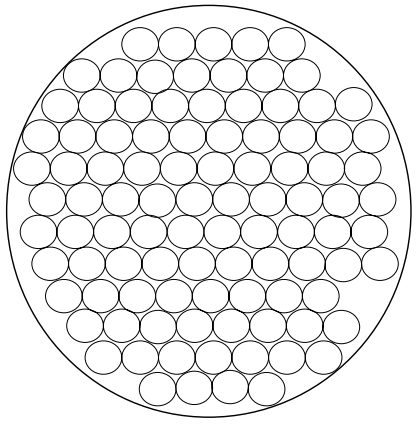
\includegraphics[width=0.5\textwidth]{./figures/chapter7/sphere_picking.png}
\end{figure}

如上图所示, 假设每一个小球的球心为一个codeword, 球的范围为可以decode到该codeword的所有码字(jointly AEP). 假设这些小球的半径为$r$, 则一个$n$为球的体积可以写为$\Vol=C_nr^n$. 由于 noise的方差为$N$, 所以小球的半径为 $\sqrt{n(n+\epsilon)}$, 而$Y$的方差为$\mathbb{E}(Y^2)=\mathbb{E}((X+Z)^2)=\mathbb{E}(X^2)+\mathbb{E}(Z^2)=P+N$, 所以整个大球的半径为$\sqrt{n(P+N)}$. 因此最多有 $\dfrac{C_n(\sqrt{n(P+N)})^n}{C_n(\sqrt{n(n+\epsilon)})^n}=\left(1+\dfrac{P}{N}\right)^{\frac{1}{2}}$ 个小球. 所以rate of the code(小球数量需要的bit数) is $\log \left(1+\dfrac{P}{N}\right)^{\frac{1}{2}}=\dfrac{1}{2}\log\left(1+\dfrac{P}{N}\right)$.

关于大球的半径大小: typical set的大小为$\Vol\left(A_{\epsilon}^{(n)}(f_Y)\right)=2^{n(H(Y))}\leq 2^{n(\frac{1}{2}\log(2\pi e (P+N)))}$, 所以半径取 $\sqrt{n(P+N)}$. 小球的半径同理.

严谨证明:
1. 可达性证明: 大致和先前证明信道容量的方法类似, 要证明$\forall R<C=I(X;Y)$时, 发生错误的概率 $P_e^{(n)}\to 0$.

通过构建码本, $X_i(w)$ 表示 码字$w$的第$i$个bit. 其中 $X_i(w)\stackrel{i.i.d.}{\sim} \mathcal{N}(0, P-\epsilon)$.

和先前一样, W.L.O.G. 令w=1, 则 $P_e^{(n)}=\Pr\left(\hat{W}\neq 1|W=1\right)$, 然后分类讨论不符合要求的情况即可. \textcolor{red}{不同之处: 增加了$E_0:\dfrac{1}{n}\sum\limits_{j=1}^n X_j(1)>P$(不满足功率约束限制)的情况}.

摆烂了, 放图片了.
\begin{figure}[htbp]
    \centering
    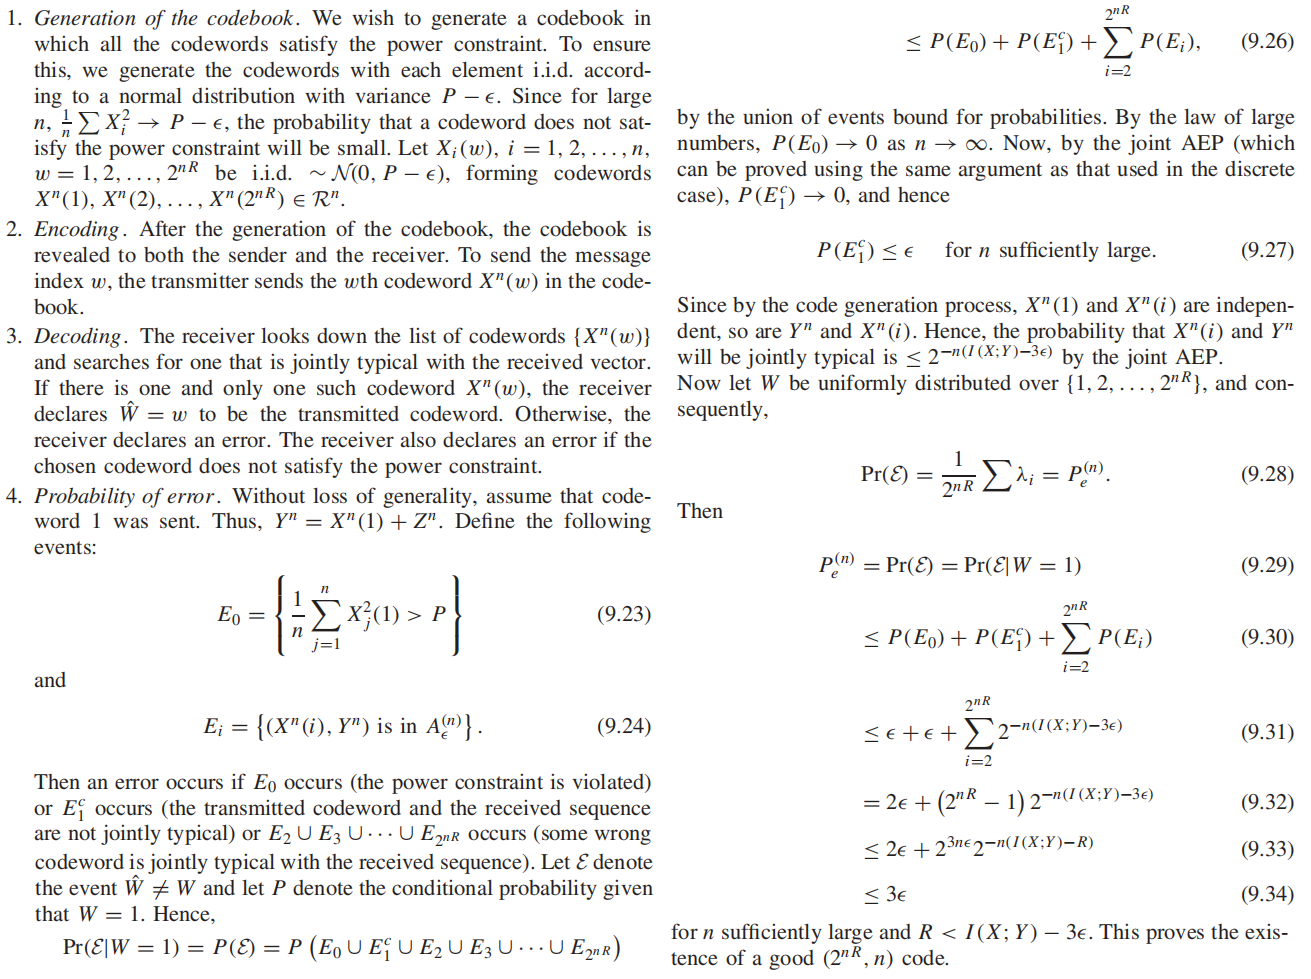
\includegraphics[width=1.25\textwidth]{./figures/chapter7/achievability.png}
\end{figure}

想要$P_e^{(n)}\to 0$, 则需要$2^{-n(I(X;Y)-R-3\epsilon)}\to 0$, i.e. $R<I(X;Y)-3\epsilon$. 这里所有提到的$I(X;Y)$都是$\max\limits_{p(x)}I(X;Y)=\frac{1}{2}\log \left(1+\frac{P}{N}\right)$.

2. Converse proof: \\
证明$\forall R>C=\frac{1}{2}\log\left(1+\frac{P}{N}\right)$时, $P_e^{(n)}\not\to 0$ with $\mathbb{E}(X^2)\leq P$. \\
同样要用 Fano's Inequality, 对于信息传递的Markov Chain $W\to X\to Y\to \hat{W}$, 有
$$H(W|\hat{W})\leq 1 + P_e^{(n)}\log 2^{nR} = 1 + P_e^{(n)}nR \triangleq n\epsilon_n$$

\begin{figure}[htbp]
    \centering
    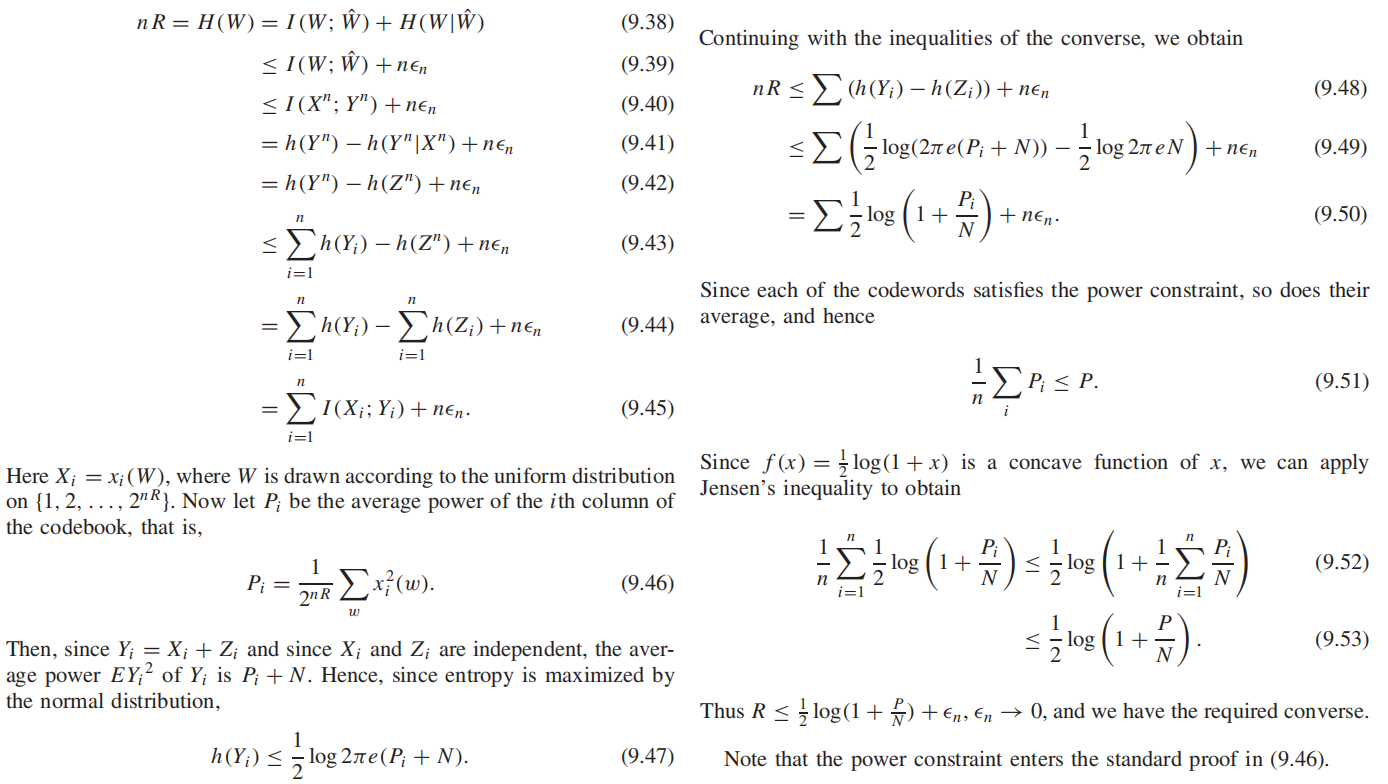
\includegraphics[width=1.25\textwidth]{./figures/chapter7/converse.png}
\end{figure}
$$R\leq \dfrac{1}{2}\log\left(1+\dfrac{P}{N}\right)+\epsilon_n=\dfrac{1}{2}\log\left(1+\dfrac{P}{N}\right)+\dfrac{1}{n}+P_e^{(n)}R$$
当$R>C=\dfrac{1}{2}\log\left(1+\dfrac{P}{N}\right)$时, 有$\dfrac{1}{n}+P_e^{(n)}R>0$, 由于$n,R$均为常数, 所以一定有$P_e^{(n)}\not\to 0$.